% !TEX TS-program = pdflatex
% !TEX encoding = UTF-8 Unicode

% This is a simple template for a LaTeX document using the "article" class.
% See "book", "report", "letter" for other types of document.

\documentclass[11pt]{article} % use larger type; default would be 10pt

%%%% \documentclass[11pt]{article} % use larger type; default would be 10pt

\usepackage[utf8]{inputenc} % set input encoding (not needed with XeLaTeX)

%%% Examples of Article customizations
% These packages are optional, depending whether you want the features they provide.
% See the LaTeX Companion or other references for full information.

%%% PAGE DIMENSIONS
\usepackage{geometry} % to change the page dimensions
\geometry{a4paper} % or letterpaper (US) or a5paper or....
% \geometry{margin=2in} % for example, change the margins to 2 inches all round
% \geometry{landscape} % set up the page for landscape
%   read geometry.pdf for detailed page layout information

\usepackage{graphicx} % support the \includegraphics command and options

% \usepackage[parfill]{parskip} % Activate to begin paragraphs with an empty line rather than an indent

%%% PACKAGES
\usepackage{booktabs} % for much better looking tables
\usepackage{array} % for better arrays (eg matrices) in maths
\usepackage{paralist} % very flexible & customisable lists (eg. enumerate/itemize, etc.)
\usepackage{verbatim} % adds environment for commenting out blocks of text & for better verbatim
\usepackage{subfig} % make it possible to include more than one captioned figure/table in a single float
% These packages are all incorporated in the memoir class to one degree or another...

\usepackage{tikz}
%% pour le diag P-V
\usetikzlibrary{decorations.markings, arrows, arrows.meta}
\tikzset{
    midar/.style 2 args={
        very thick,
        decoration={name=markings,
        mark=at position .55 with {\arrow{latex}},
        mark=at position 0 with {\fill circle (2pt);},
        mark=at position 1 with {\fill circle (2pt);}}
        ,postaction=decorate,
    },
}
%% pour la machine
\usetikzlibrary{shapes,arrows}
\tikzset{%
pics/.cd,
nodea/.style args={#1#2#3}{
  code={\node[minimum height=2cm] (#3) {\color{#1}#2};
       \draw[thick] (#3.south west) -| (#3.north east)--(#3.north west);
  }
},
%pics/.cd,
nodeb/.style args={#1#2#3}{
  code={\node[minimum height=2cm] (#3) {\color{#1}#2};
       \draw[thick] (#3.south east) -| (#3.north west)--(#3.north east);
  }
},
%pics/.cd,
nodec/.style args={#1#2#3}{
  code={\node[draw,thick,shape=circle,inner sep=1cm] (#3) {\color{#1}#2};
  }
},
}
%% pour http://texample.net/media/tikz/examples/TEX/is-lm-diagram.tex
\usetikzlibrary{arrows,calc}
\usepackage{relsize}
\newcommand\LM{\ensuremath{\mathit{LM}}}
\newcommand\IS{\ensuremath{\mathit{IS}}}
%% pour...

%%% HEADERS & FOOTERS
\usepackage{fancyhdr} % This should be set AFTER setting up the page geometry
\pagestyle{fancy} % options: empty , plain , fancy
\renewcommand{\headrulewidth}{0pt} % customise the layout...
\lhead{}\chead{}\rhead{}
\lfoot{}\cfoot{\thepage}\rfoot{}

%%% SECTION TITLE APPEARANCE
\usepackage{sectsty}
\allsectionsfont{\sffamily\mdseries\upshape} % (See the fntguide.pdf for font help)
% (This matches ConTeXt defaults)

%%% ToC (table of contents) APPEARANCE
\usepackage[nottoc,notlof,notlot]{tocbibind} % Put the bibliography in the ToC
\usepackage[titles,subfigure]{tocloft} % Alter the style of the Table of Contents
\renewcommand{\cftsecfont}{\rmfamily\mdseries\upshape}
\renewcommand{\cftsecpagefont}{\rmfamily\mdseries\upshape} % No bold!

%%% The "real" document content comes below...


%%% The "real" document content comes below...

\title{La thermodynamique à la plage}
\author{Jean-Louis Dufour}
%\date{} % Activate to display a given date or no date (if empty),
         % otherwise the current date is printed 

\begin{document}
\maketitle

You do not know anything until you have practiced.
R. Feynman

There is no Royal Road to geometry
Euclid's reply to king Ptolemy's request for 'The Elements for dummies' (according to Proclus)

I hear and I forget. I see and I remember. I do and I understand.
Confucius

\section{Introduction}

Euclide (-330 - -270) enseigna à Alexandrie sous Ptolémée Iier Sôter.

Paul Tannery, la géométrie grecque (1887), p.69 :

Euclide vivait sous Ptolémée I ...
on rapporte que Ptolémée demanda un jour à Euclide
s'il n’y avait pas pour la Géométrie de route plus courte que celle des Éléments;
il eut cette réponse : " Il n’y a pas en Géométrie de chemin fait pour les rois ".

Alexis-Claude Clairaut (1713-1765)
1740 : Mémoire sur l'intégration ou la construction des équations différentielles du premier ordre






\section{Pression et Température}

Une masse de $1~kg$ donne lieu sur Terre à une \emph{force} vers le centre de la Terre d'environ $9.8~N$ (c'est ce qu'on appelle le 'poids', et c'est en général via le poids qu'on mesure la masse).
Lorsque je monte sur ma balance, je fais peser $75~kg * 9.8~N/kg \approx 750~N $ sur une surface d'environ $2*25~cm*5~cm = 250~cm^2 = 2.5~dm^2 = 2.5~10^{-2}~m^2$. Un physicien dira que j'exerce sur la balance une \emph{pression}
$$
P = \frac{750~N}{2.5~10^{-2}~m^2} = 3~10^4 N/m^2 
$$
L'unité SI de pression étant le \emph{Pascal}, cela fait $30~kPa$

pourquoi le Pascal ? -> bla sur le creve-tonneau

\section{Boyle}

% BEGIN BENSON
En 1662, Robert Boyle

%END BENSON

\section{Python}

cantera, Dave Goodwin \& coll., cantera.org, conda create --name spam --channel cantera cantera ipython matplotlib

thermo, Caleb Bell, thermo.readthedocs.io, conda install -c conda-forge thermo

pyromat, Christopher Martin, pyromat.org, pip install pyromat





\section{Figures diverses}

figure -1

\begin{tikzpicture}[domain=0:4]
\draw[color=orange] plot (\x,{\x / 4}) node[right] {$f(x) = 4 / x$};
\end{tikzpicture}

figure 0

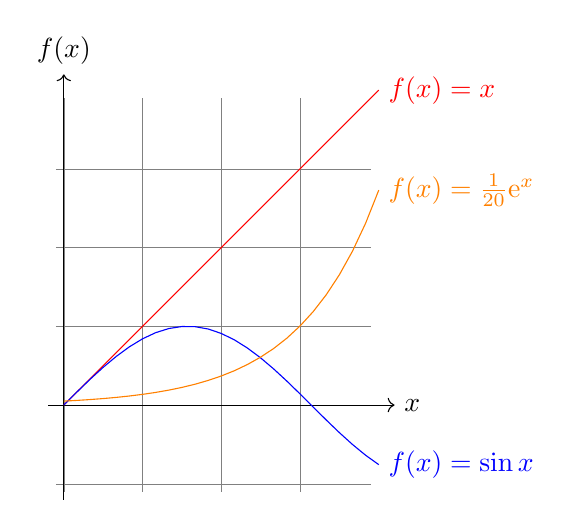
\begin{tikzpicture}[domain=0:4]
\draw[very thin,color=gray] (-0.1,-1.1) grid (3.9,3.9);
\draw[->] (-0.2,0) -- (4.2,0) node[right] {$x$};
\draw[->] (0,-1.2) -- (0,4.2) node[above] {$f(x)$};
\draw[color=red] plot (\x,\x) node[right] {$f(x) =x$};
% \x r means to convert '\x' from degrees to _r_adians:
\draw[color=blue] plot (\x,{sin(\x r)}) node[right] {$f(x) = \sin x$};
\draw[color=orange] plot (\x,{0.05*exp(\x)}) node[right] {$f(x) = \frac{1}{20} \mathrm e^x$};
\end{tikzpicture}

figure 1

\begin{tikzpicture}
\draw (0,0) --(1,2);
\end{tikzpicture}

figure 2

\begin{tikzpicture}[xscale=25,yscale=5]
\draw [<->, help lines] (0.6,1.34) -- (0.6,1) -- (1.05,1);
\draw[orange] (0.6, 1.0385) --
(0.61, 1.06372) -- (0.62, 1.08756) -- (0.63, 1.11012) -- (0.64,
1.13147) -- (0.65, 1.15166) -- (0.66, 1.17074) -- (0.67, 1.18874) -- (0.68,
1.20568) -- (0.69, 1.22157) -- (0.7, 1.23643) -- (0.71, 1.25026) -- (0.72,
1.26307) -- (0.73, 1.27486) -- (0.74, 1.28561) -- (0.75, 1.29534) -- (0.76,
1.30402) -- (0.77, 1.31165) -- (0.78, 1.31821) -- (0.79, 1.32369) -- (0.8,
1.32806) -- (0.81, 1.33131) -- (0.82, 1.3334) -- (0.83, 1.33431) -- (0.84,
1.334) -- (0.85, 1.33244) -- (0.86, 1.32956) -- (0.87, 1.32533) -- (0.88,
1.31966) -- (0.89, 1.3125) -- (0.9, 1.30373) -- (0.91, 1.29325) -- (0.92,
1.2809) -- (0.93, 1.26649) -- (0.94, 1.24976) -- (0.95, 1.23032) -- (0.96,
1.2076) -- (0.97, 1.18065) -- (0.98, 1.14763) -- (0.99, 1.1038) -- (0.991,
1.09836) -- (0.992, 1.09261) -- (0.993, 1.0865) -- (0.994, 1.07994) -- (0.995,
1.07282) -- (0.996, 1.06497) -- (0.997, 1.0561) -- (0.998, 1.04563) -- (0.999,
1.03209) -- (0.9991, 1.03042) -- (0.9992, 1.02866) -- (0.9993,
1.02679) -- (0.9994, 1.02478) -- (0.9995, 1.0226) -- (0.9996, 1.02019) -- (0.9997,
1.01747) -- (0.9998, 1.01424) -- (0.9999, 1.01005) -- (0.9999,
1.01005) -- (0.99991, 1.00953) -- (0.99992, 1.00898) -- (0.99993,
1.0084) -- (0.99994, 1.00778) -- (0.99995, 1.0071) -- (0.99996,
1.00634) -- (0.99997, 1.00549) -- (0.99998, 1.00448) -- (0.99999, 1.00317) -- (1,
1) ;
\end{tikzpicture}

figure 3

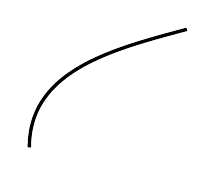
\begin{tikzpicture}
\draw[very thick] (0,0) to [out=90,in=195] (2,1.5);
\end{tikzpicture}

figure 4

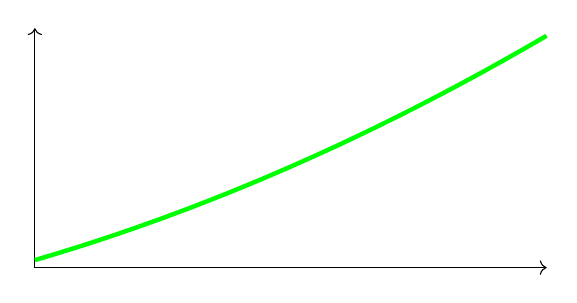
\begin{tikzpicture}[xscale=13,yscale=3.8]
\draw [<->] (0,0.8) -- (0,0) -- (0.5,0);
\draw[green, ultra thick, domain=0:0.5] plot (\x, {0.025+\x+\x*\x});
\end{tikzpicture}

figure 5

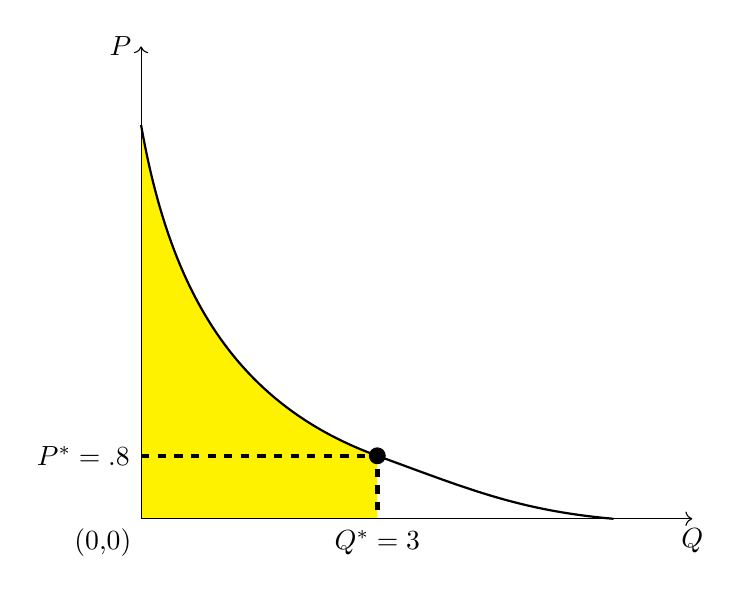
\begin{tikzpicture}
\path [fill=yellow] (0,0) -- (0,5) to [out=-80, in=160]
(3,.8) -- (3,0) -- (0,0);
\draw [<->] (0,6) node [left] {$P$} -- (0,0)
node [below left] {(0,0)} -- (7,0) node [below] {$Q$};
\draw [ultra thick, dashed] (0,.8) node [left] {$P^*=.8$} -- (3,.8)
-- (3,0) node [below] {$Q^*=3$};
\draw [fill] (3,.8) circle [radius=.1];
\draw [thick] (0,5) to [out=-80, in=160] (3,.8) to
[out=-20, in=175] (6,0);
\end{tikzpicture}

figure 6

%\begin{center}
\begin{tikzpicture}[domain=0:0.5,xscale=13,yscale=3.8]
\draw[<->] (0,2) node[left]{EUR}-- (0,0) -- (.7,0) node[below] {$q$};
\draw[red] plot (\x, {0.25+\x/2+\x*\x/2}) node[right] {$v_1(x)$};
\draw[green] plot (\x, {0.025+\x+\x*\x}) node[right] {$v_2(x)$};
\draw[thin, dashed] plot (\x, {0.275+1.5*\x+1.5*\x*\x}) ;
\draw[thick,domain=0:0.33666] plot (\x, {0.05+2*\x+2*\x*\x}) ;
\draw[thick,domain=0.33666:0.5]
plot (\x, {0.5+\x+\x*\x}) node[right] {$2\min[v_1,v_2]$};
\end{tikzpicture}
%\end{center}

figure 7

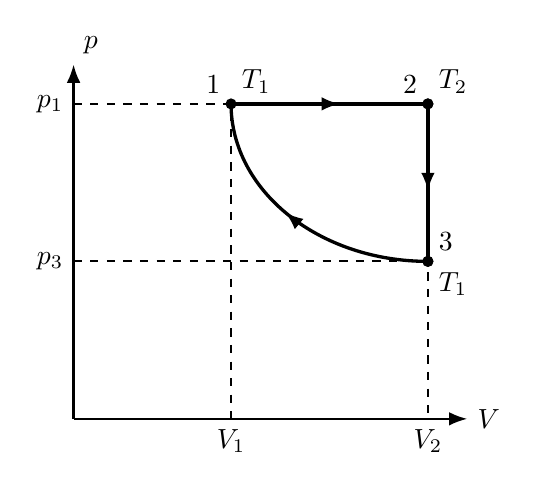
\begin{tikzpicture}[thick]
    \draw[-{Latex}] (0,0) -- (0,4.5) node[above right] {$p$};
    \draw[-{Latex}] (0,0) -- (5,0) node[right] {$V$};

    \draw[dashed] (0,4) node[left] {$p_{1}$} -| (2,0) node[below] {$V_{1}$};
    \draw[dashed] (0,2) node[left] {$p_{3}$} -| (4.5,0) node[below] {$V_{2}$};

\draw[midar] (2,4) node[above left]{1} node[above right]{$T_1$} -- 
    (4.5,4) node[above left]{2} node[above right]{$T_2$};   
\draw[midar] (4.5,4) -- (4.5,2) node[above right]{3} node[below right]{$T_1$};
\draw[midar] (4.5,2) arc (270:180:2.5 and 2);
\end{tikzpicture}

figure 8

  \begin{tikzpicture}[scale=2]
    \pic at (0,0) {nodea={red}{$T_H$}{L}};
    \pic at (2,0) {nodec={black}{}{C}};
    \pic at (4,0) {nodeb={blue}{$T_C$}{R}};
 \draw[->,>=latex](L)--node[midway,above]{$\mathbf{Q_H}$}(C); 
 \draw[->,>=latex](C)--node[midway,above]{$\mathbf{Q_C}$} (R);
 \draw[->,>=latex](C)--node[midway,left]{$\mathbf{W}$} ++(0,-2cm);
  \end{tikzpicture}

figure 9

%%  http://texample.net/media/tikz/examples/TEX/colored-diagram.tex

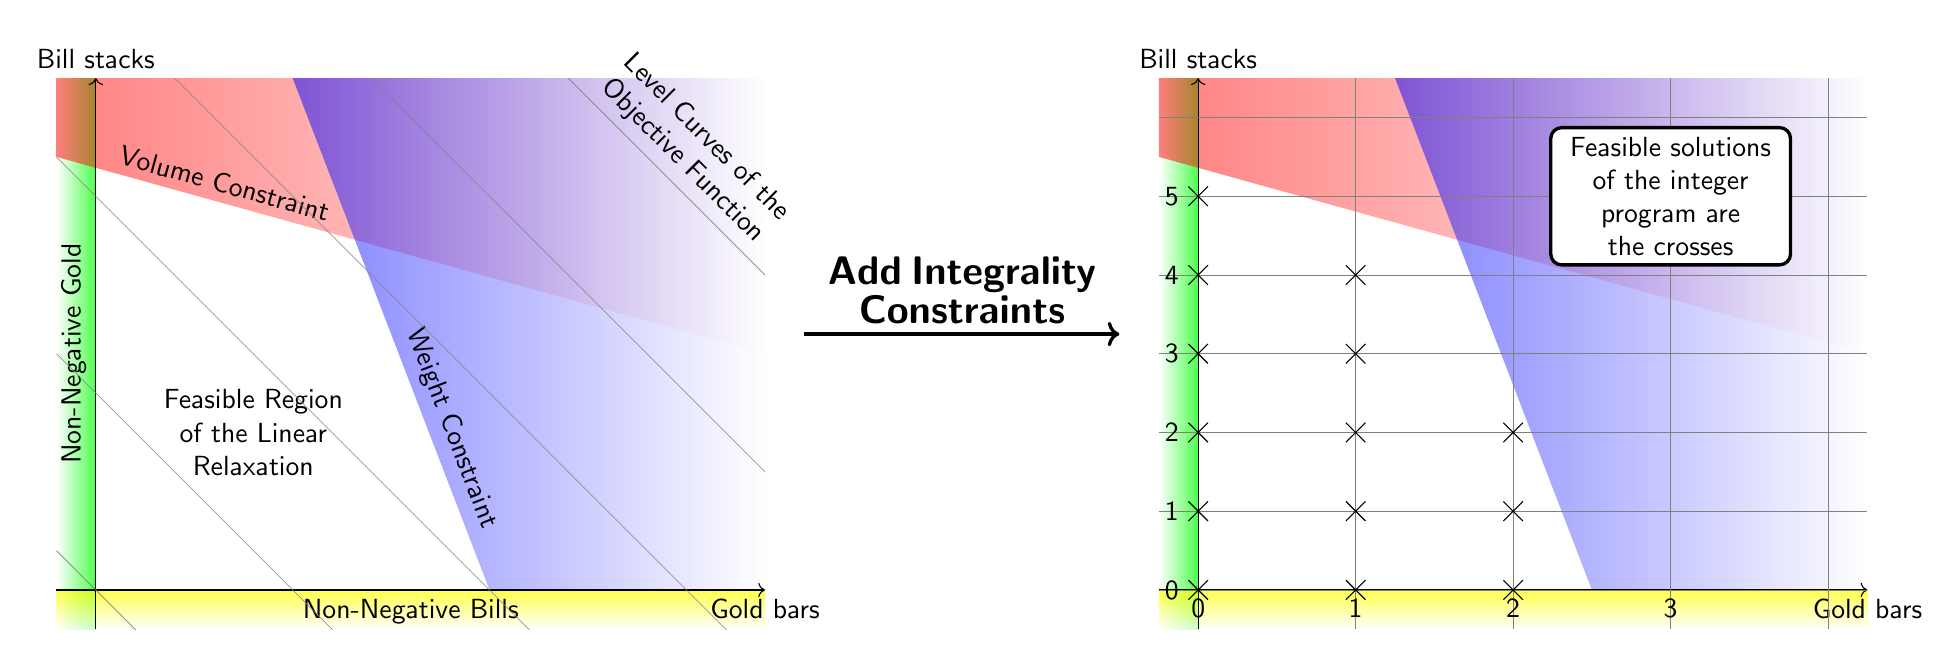
\begin{tikzpicture}[
    every path/.style = {},
    every node/.append style = {font=\sffamily}
  ]
  \begin{scope}
    \shade[right color=green, left color=white, opacity=0.7]
      (-0.5,-0.5) rectangle (0,6.5);
    \node[rotate=90, above] at (0,3) {Non-Negative Gold};
    \shade[top color=yellow, bottom color=white, opacity=0.7]
      (-0.5,-0.5) rectangle (8.5,0);
    \node[below] at (4,0) {Non-Negative Bills};
    \shade[left color=red, bottom color=red, right color=white, opacity=0.5]
      (-0.5,5.5) -- (8.5,3) -- (8.5,6.5) -- (-0.5,6.5) -- cycle;
    \path (-0.5,5.5) -- node[pos=0.23, sloped, above] {Volume Constraint}
      (8.5,3);
    \shade[left color=blue, right color=white, opacity=0.5]
      (2.5,6.5) -- (8.5,6.5) -- (8.5,0) -- (5,0) -- cycle;
    \path (5,0) -- node[pos=0.3, sloped, above] {Weight Constraint} (2.5,6.5);
    \node[text width=7em, align=center] at (2,2)
      {Feasible Region of the Linear Relaxation};
    \draw[->] (-0.5,0) -- (8.5,0) node[below] {Gold bars};
    \draw[->] (0,-0.5) -- (0,6.5) node[above] {Bill stacks};
    \node[rotate=-45, above, text width=9em, align=center] at (7.25,5.25)
      {Level Curves of the Objective Function};
    \path[clip] (-0.5,-0.5) rectangle (8.5,6.5);
    \foreach \i in {0.5,3,...,13} {
      \draw[help lines] (-0.5,\i) -- +(-45:15);
    }
  \end{scope}
  \draw[very thick, ->] (9,3.25) -- node[above, text width=4cm, align=center]
    {\Large\bfseries Add Integrality Constraints} (13,3.25);
  \begin{scope}[shift={(14,0)}]
    \shade[right color=green, left color=white, opacity=0.7]
      (-0.5,-0.5) rectangle (0,6.5);
    \shade[top color=yellow, bottom color=white, opacity=0.7]
      (-0.5,-0.5) rectangle (8.5,0);
    \shade[left color=red, bottom color=red, right color=white, opacity=0.5]
      (-0.5,5.5) -- (8.5,3) -- (8.5,6.5) -- (-0.5,6.5) -- cycle;
   \shade[left color=blue, right color=white, opacity=0.5]
     (2.5,6.5) -- (8.5,6.5) -- (8.5,0) -- (5,0) -- cycle;
    \draw[->] (-0.5,0) -- (8.5,0) node[below] {Gold bars};
    \draw[->] (0,-0.5) -- (0,6.5) node[above] {Bill stacks};
    \foreach \i in {0,1,...,6.5} {
      \draw[help lines] (-0.5,\i) -- (8.5,\i);
    }
    \foreach \i in {2,4,...,8.5} {
      \draw[help lines] (\i,6.5) -- (\i,-0.5);
    }
    \foreach \i in {0,1,...,5} {
      \node[draw,cross out,label={left:\i}] at (0,\i) {};
    }
    \foreach \i in {0,1,...,4} {
      \node[draw,cross out] at (2,\i) {};
    }
    \foreach \i in {0,1,...,2} {
            \node[draw,cross out] at (4,\i) {};
    }
    \foreach \i in {0,2,...,6} {
      \node[below] at (\i,0) {\pgfmathparse{int(\i/2)}\pgfmathresult};
    }
    \node[very thick, draw=black, fill=white, rectangle, rounded corners,
      text width=8em, align=center] at (6,5)
      {Feasible solutions of the integer program are the crosses};
  \end{scope}
\end{tikzpicture}

figure 10

%% http://texample.net/media/tikz/examples/TEX/is-lm-diagram.tex

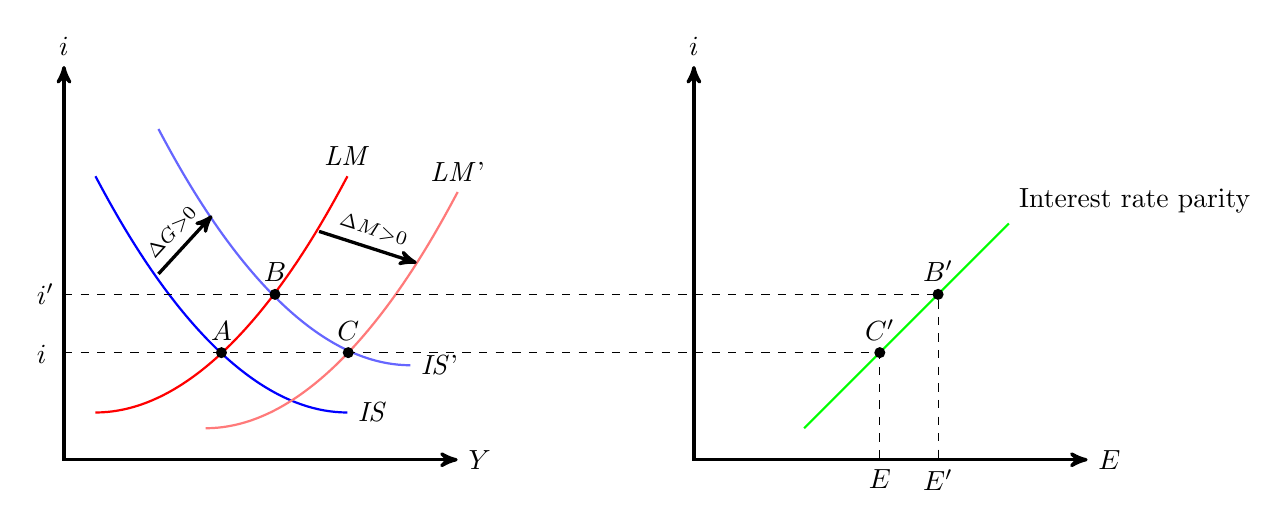
\begin{tikzpicture}[
        scale=2,
        IS/.style={blue, thick},
        LM/.style={red, thick},
        axis/.style={very thick, ->, >=stealth', line join=miter},
        important line/.style={thick}, dashed line/.style={dashed, thin},
        every node/.style={color=black},
        dot/.style={circle,fill=black,minimum size=4pt,inner sep=0pt,
            outer sep=-1pt},
    ]
    % axis
    \draw[axis,<->] (2.5,0) node(xline)[right] {$Y$} -|
                    (0,2.5) node(yline)[above] {$i$};
    % IS-LM diagram
    \draw[LM] (0.2,0.3) coordinate (LM_1) parabola (1.8,1.8)
        coordinate (LM_2) node[above] {\LM};
    \draw[IS] (0.2,1.8) coordinate (IS_1) parabola[bend at end]
         (1.8,.3) coordinate (IS_2) node[right] {\IS};
    %Intersection is calculated "manually" since Tikz does not offer
    %intersection calculation for parabolas
    \node[dot,label=above:$A$] at (1,.68) (int1) {};
    %shifted IS-LM diagram
    \draw[xshift=.7cm, LM, red!52] (0.2,0.2) parabola (1.8,1.7)
        node[above] {\LM'};
    \draw[xshift=.4cm, yshift=.3cm, IS, blue!60] (0.2,1.8)
        parabola[bend at end] (1.8,.3)
        node[right] {\IS'};
    %Intersection of shifted IS-LM
    \path[xshift=.36cm, yshift=.35cm] (.98,.7)
        node[dot,label=above:{$B$}] (int2) {};
    \path[xshift=.805cm] (1,.68) node[dot,label=above:$C$] (int3) {};
    %arrows between intersections
    \draw[->, very thick, black, >=stealth']
        ($(int1)+1/2*(-.80,1)$) -- ($(int2)+1/2*(-.8,1)$)
        node[sloped, above, midway] {$\mathsmaller{\Delta G > 0}$};
    \draw[->, very thick, black, >=stealth']
        ($(int2)+2*(.14,.2)$) -- ($(int2)!.2cm!270:(int2)+(.9,0)$)
        node[sloped,above, midway] {$\mathsmaller{\Delta M>0}$};
        
    \begin{scope}[xshift=4cm]
        %E-diagram
        \draw[axis,<->] (0,2.5) node(eyline)[above] {$i$} |-
                        (2.5,0) node(exline)[right] {$E$};

        \draw[important line, green, xshift=.5cm]
            (.2,.2) coordinate (es) -- (1.5,1.5) coordinate (ee)
            node [above right] {Interest rate parity};
    \end{scope}
    %Lines connecting IS LM coordinates and E coordinates
    \draw[dashed] 
        let
            % Store the intersection point in \p1 for later retrieval. 
            % A convenient feature of the let operation is that we can
            % access the x and y component of the coordinate directly 
            % using the \x1 and \y1 syntax. 
            \p1=(intersection of int2--[xshift=1]int2 and es--ee)
        in
            (0,\y1) node[left]{$i'$} -|  (\x1,0)
            node[pos=0.5,dot,label=above:$B'$] {} node[below] {$E'$};

    \draw[dashed line] let
        \p1=(intersection of int3--[xshift=1]int3 and es--ee)
            in
        (0,\y1) node[left]{$i\phantom{'}$} -| (\x1,0)
        node[dot,label=above:$C'$,pos=0.5] {} node[below] {$E$};

\end{tikzpicture}

figure 11

%% http://texample.net/media/tikz/examples/TEX/parallel-lines.tex

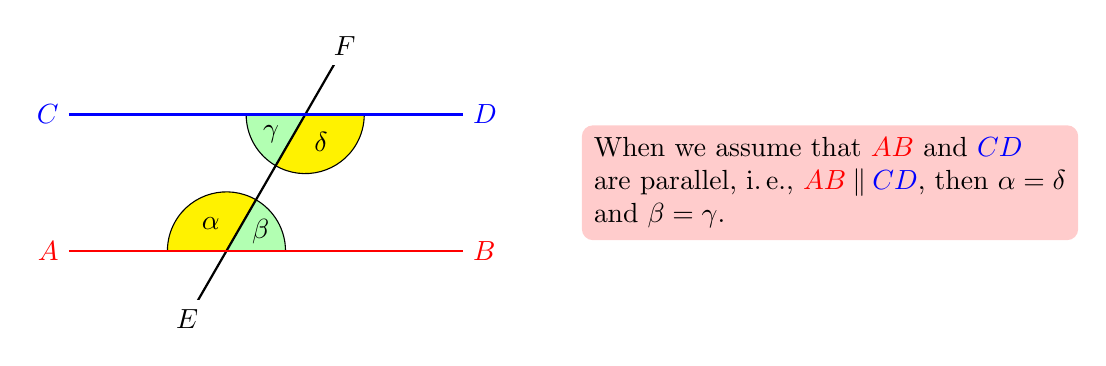
\begin{tikzpicture}
  \draw[fill=yellow] (0,0) -- (60:.75cm) arc (60:180:.75cm);
  \draw(120:0.4cm) node {$\alpha$};

  \draw[fill=green!30] (0,0) -- (right:.75cm) arc (0:60:.75cm);
  \draw(30:0.5cm) node {$\beta$};

  \begin{scope}[shift={(60:2cm)}]
    \draw[fill=green!30] (0,0) -- (180:.75cm) arc (180:240:.75cm);
    \draw (30:-0.5cm) node {$\gamma$};

    \draw[fill=yellow] (0,0) -- (240:.75cm) arc (240:360:.75cm);
    \draw (-60:0.4cm) node {$\delta$};
  \end{scope}

  \begin{scope}[thick]
    \draw (60:-1cm) node[fill=white] {$E$} -- (60:3cm) node[fill=white] {$F$};
    \draw[red]                   (-2,0) node[left] {$A$} -- (3,0) 
                                        node[right]{$B$};
    \draw[blue,shift={(60:2cm)}] (-3,0) node[left] {$C$} -- (2,0) 
                                        node[right]{$D$};
  
    \draw[shift={(60:1cm)},xshift=4cm]
    node [right,text width=6cm,rounded corners,fill=red!20,inner sep=1ex]
    {
      When we assume that $\color{red}AB$ and $\color{blue}CD$ are
      parallel, i.\,e., ${\color{red}AB} \mathbin{\|} \color{blue}CD$,
      then $\alpha = \delta$ and $\beta = \gamma$.
    };
  \end{scope}
\end{tikzpicture}

figure 12

%% http://texample.net/media/tikz/examples/TEX/bisector.tex

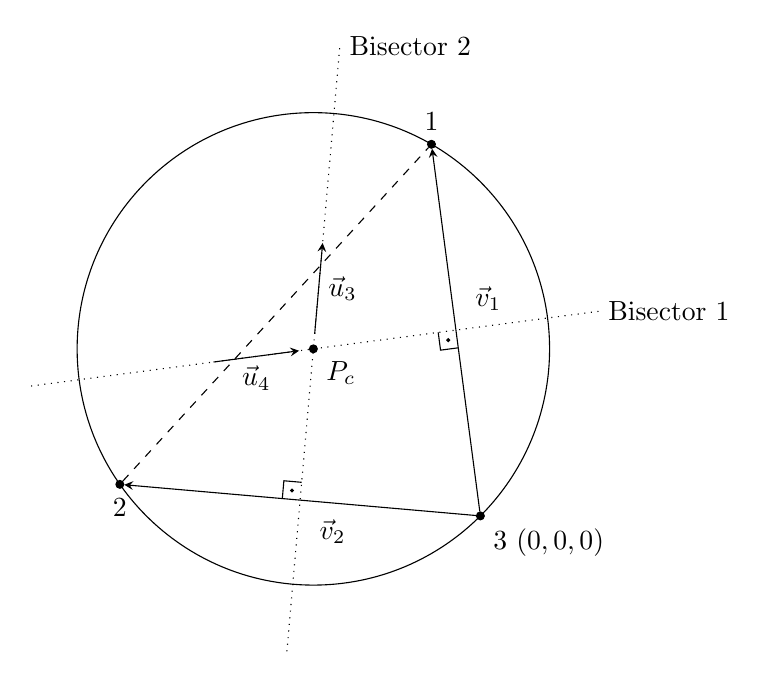
\begin{tikzpicture}
  [
    scale=3,
    >=stealth,
    point/.style = {draw, circle,  fill = black, inner sep = 1pt},
    dot/.style   = {draw, circle,  fill = black, inner sep = .2pt},
  ]

  % the circle
  \def\rad{1}
  \node (origin) at (0,0) [point, label = {below right:$P_c$}]{};
  \draw (origin) circle (\rad);

  % triangle nodes: just points on the circle
  \node (n1) at +(60:\rad) [point, label = above:$1$] {};
  \node (n2) at +(-145:\rad) [point, label = below:$2$] {};
  \node (n3) at +(-45:\rad) [point, label = {below right:$3$ $(0, 0, 0)$}] {};

  % triangle edges: connect the vertices, and leave a node at the midpoint
  \draw[->] (n3) -- node (a) [label = {above right:$\vec{v}_1$}] {} (n1);
  \draw[->] (n3) -- node (b) [label = {below right:$\vec{v}_2$}] {} (n2);
  \draw[dashed] (n2) -- (n1);

  % Bisectors
  % start at the point lying on the line from (origin) to (a), at
  % twice that distance, and then draw a path going to the point on
  % the line lying on the line from (a) to the (origin), at 3 times
  % that distance.
  \draw[dotted]
    ($ (origin) ! 2 ! (a) $)
    node [right] {Bisector 1}
    -- ($(a) ! 3 ! (origin)$ );

  % similarly for origin and b
  \draw[dotted]
    ($ (origin) ! 2 ! (b) $)
    -- ($(b) ! 3 ! (origin)$ )
    node [right] {Bisector 2};

  % short vectors
  \draw[->]
    ($ (origin) ! -.7 ! (a) $)
    -- node [below] {$\vec{u}_4$}
    ($ (origin) ! -.1 ! (a) $);
  \draw[->]
    ($ (origin) ! -.1 ! (b) $)
    -- node [right] {$\vec{u}_3$}
    ($ (origin) ! -.7 ! (b) $);

  % Right angle symbols
  \def\ralen{.5ex}  % length of the short segment
  \foreach \inter/\first/\last in {a/n3/origin, b/n2/origin}
    {
      \draw let \p1 = ($(\inter)!\ralen!(\first)$), % point along first path
                \p2 = ($(\inter)!\ralen!(\last)$),  % point along second path
                \p3 = ($(\p1)+(\p2)-(\inter)$)      % corner point
            in
              (\p1) -- (\p3) -- (\p2)               % path
              ($(\inter)!.5!(\p3)$) node [dot] {};  % center dot
    }
\end{tikzpicture}

figure 13

\end{document}
